\documentclass[12pt]{report}
\usepackage{graphicx}
\usepackage{tikz}
\usepackage{changepage} 
\usepackage{./tikz-uml}
\usepackage[section]{placeins}
\usepackage[english]{babel}
\usepackage{amsmath}
\usepackage{latexsym}
\usepackage{amsfonts}
\usepackage[normalem]{ulem}
\usepackage{array}
\usepackage{amssymb}
\usepackage[left=0.75in,right=0.75in,top=1.5in,bottom=1.5in,footskip=.25in]{geometry}
\usepackage[utf8]{inputenc}
\usepackage[toc,automake,acronym,section]{glossaries}
\usepackage[backend=biber,
style=numeric,
sorting=none,
isbn=false,
doi=false,
url=false,
]{biblatex}\addbibresource{bibliography.bib}
\usepackage{subfig}
\usepackage{wrapfig}
\usepackage{wasysym}
\usepackage{enumitem}
\usepackage{adjustbox}
\usepackage{./ragged2e}
\usepackage{longtable}
\usepackage{setspace}
\usepackage{hhline}
\usepackage{multicol}
\usepackage{./tabto}
\usepackage{float}
\usepackage{multirow}
\usepackage{makecell}
\usepackage{fancyhdr}
\usepackage[toc,page]{appendix}
\usepackage[hidelinks]{hyperref}
\usetikzlibrary{shapes.symbols,shapes.geometric,shadows,arrows.meta}
\tikzset{>={Latex[width=1.5mm,length=2mm]}}
\usepackage{flowchart}
\usepackage[utf8]{inputenc}
\usepackage[T1]{fontenc}
\TabPositions{0.5in,1.0in,1.5in,2.0in,2.5in,3.0in,3.5in,4.0in,4.5in,5.0in,5.5in,6.0in,}

\urlstyle{same}
\setcounter{tocdepth}{5}
\setcounter{secnumdepth}{5}

\setlistdepth{9}
\renewlist{enumerate}{enumerate}{9}
		\setlist[enumerate,1]{label=\arabic*)}
		\setlist[enumerate,2]{label=\alph*)}
		\setlist[enumerate,3]{label=(\roman*)}
		\setlist[enumerate,4]{label=(\arabic*)}
		\setlist[enumerate,5]{label=(\Alph*)}
		\setlist[enumerate,6]{label=(\Roman*)}
		\setlist[enumerate,7]{label=\arabic*}
		\setlist[enumerate,8]{label=\alph*}
		\setlist[enumerate,9]{label=\roman*}

\renewlist{itemize}{itemize}{9}
		\setlist[itemize]{label=$\cdot$}
		\setlist[itemize,1]{label=\textbullet}
		\setlist[itemize,2]{label=$\circ$}
		\setlist[itemize,3]{label=$\ast$}
		\setlist[itemize,4]{label=$\dagger$}
		\setlist[itemize,5]{label=$\triangleright$}
		\setlist[itemize,6]{label=$\bigstar$}
		\setlist[itemize,7]{label=$\blacklozenge$}
		\setlist[itemize,8]{label=$\prime$}

\setlength{\topsep}{0pt}\setlength{\parskip}{9.96pt}
\setlength{\parindent}{0pt}

\renewcommand{\arraystretch}{1.3}

\newglossaryentry{igo}
{
	name=iGo,
	description={The online Ticket Vending Machine integrated with STM system}
}
\newglossaryentry{membership_card}
{
	name=Membership Card,
	description={ A membership card for STM users ,convenient for daily commuters which can be recharged on monthly , weekly basis according to the card type }
}
\newglossaryentry{transaction}
{
	name=Transaction,
	description={A user's interaction with the machine to buy a rechargeable/non rechargeable ticket depending on the type selected}
}
\newglossaryentry{session}
{
	name=Session,
	description={The time allotted for each user transaction , represented by an active session}
}
\newglossaryentry{UCMiGo}
{
	name=UCMiGo,
	description={The Use case Model for user's interaction with iGo}
}
\newglossaryentry{TVM}
{
	name=TVM,
	description={Ticket Vending Machine}
}
\newglossaryentry{STM}
{
	name=STM,
	description={Société de transport de Montréal}
}



\makeglossaries


\begin{document}
	

\begin{titlepage}
	\newcommand{\HRule}{\rule{\linewidth}{0.5mm}} %New command for thickness of line	
	
	
	\centering 
	
\includegraphics[scale=.5]{logo.png}\\[1cm] 
	\textsc{\Large SOEN 6481 - SOFTWARE SYSTEMS REQUIREMENTS SPECIFICATION (FALL 2019)} \\  [0.5cm]
	
	%--------
	%	TITLE
	%--------
	
	\HRule \\[0.4cm]
	{ \huge \bfseries TICKET VENDING MACHINE}\\[0.4cm] 
	\HRule \\[0.5cm]
	
	{\large \textbf{DELIVERABLE (D1)} }	
	
	\HRule \\[1.5cm]
	%---------
	%	TAIL SECTION OF TITLE PAGE
	%---------
	\vspace{1cm}
	
	\begin{flushleft}
		
		
		\textbf{\underline{\Large Submitted By: (Team J)}}
		\hfill
		\textbf{\underline{\Large Submitted To:}} \\
		\vspace{3mm}
		\large Sanjana Udar (40094029)
		\hfill
		\large Prof. Pankaj Kamthan \\
		
		\large Raghav Verma (40076250) \hfill \\
		\large Sucheta Vijayakumar Sudhakumari (40080543) \hfill \\
		\large Hardik Vora (40087606) \hfill \\
		\large Chao Ye (40055665) \\
		
	\end{flushleft}
	
	\centering \vspace{1cm}
	
	GitHub - \href{https://github.com/hardikv21/SOEN6481.git}{https://github.com/hardikv21/SOEN6481.git}
	
	\vspace{0.1cm}
	{\large \today}\\[2cm]
	
	\vfill
\end{titlepage}


\tableofcontents
\clearpage

\chapter{Introduction}
\section{Description of TVM selected - STM}
A Ticket Vending Machine (TVM) is a kiosk that produces paper based tickets or recharges a subscription card for a particular domain. Here, we are specifically talking about a TVM for transportation services.

We have chosen the TVM that is used for Société de transport de Montréal (STM)\gls{STM} which is the enterprise that provides public bus and metro transportation services in the city of Montreal, Quebec, Canada. 

This TVM provides the users with options to get:
\begin{enumerate}
\item a one time ticket which can be a One or two way pass, 3 days pass, weekend pass.
\item Recharge the Opus card for a weekly, monthly, four-months or an yearly subscription. 
\end{enumerate}

If a user does not have an Opus card; they select the option of “Non-chargeable” and proceed with selecting the type of fare and make a payment with a debit/credit card via a payment gateway. The TVM process the payment and generates a paper based ticket and a receipt for the transaction\gls{transaction}.

If a user has an Opus card; they have to put in their Opus card in the card reader and chose the option for “Rechargeable card”. This will give them the option to choose among the possibility of recharge that they can opt for depending what their Opus card is registered under. After that, the payment is made via a payment gate way, the Opus card is recharged and the TVM generates a receipt for the transaction.  

The TVM used for STM provides service in English as well as French to cover the requirement of a Bilingual city. 
 
Every metro station in Montreal consists of one or more TVMs to make it convenient for the public to get around in the city. 




\chapter{Context of use model}


The context of use framework chosen is user centric that is it is created from the perspective of user.[1]\par


\vspace{\baselineskip}

\vspace{\baselineskip}


%%%%%%%%%%%%%%%%%%%% Figure/Image No: 1 starts here %%%%%%%%%%%%%%%%%%%%

\begin{figure}[H]
	\begin{Center}
		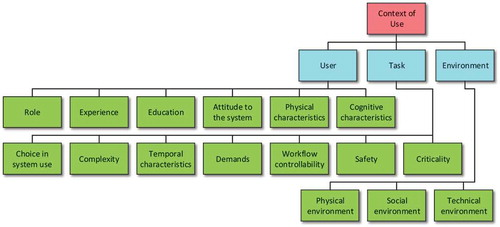
\includegraphics[width=5.21in,height=2.36in]{./p2_image1.jpeg}
	\end{Center}
	\caption{Three main aspects of context of use}
\end{figure}


%%%%%%%%%%%%%%%%%%%% Figure/Image No: 1 Ends here %%%%%%%%%%%%%%%%%%%%

\par



\section{User}

\subsection{Role}

The role of the users who wants to transit through STM will be able to recharge their monthly,weekly or daily pass.\par

The user can also book for one time transit and the user can also recharge their STM pass by paying through their debit card or by cash.\par

\subsection{Experience}

The practical skills and knowledge needed to operate the iGO\gls{igo} are basic.the user must be acquainted with making of online transactions while recharging or getting a transit ticket from the machine.also the user must be aware how to board the train or a bus by following the instructions,time and directions.\par


\subsection{Education}

The language constraints on TVM are French or English so the user must be familiar with the two languages.Since the it is a TVM which is computer and thus user must be familiar with basic operations of computer.\par

\subsection{Physical Characteristics}

The iGO will be a kiosk, thus a normal human without any disability who is able to stand can use the machine for physically handicapped,the person on wheelchair will be able to access the machine as it will be installed on an height against the wall which will be suitable for him/her to operate.The people who are blind will not be able to use the machine as there is no facility to provide reading of text on screen.\par


\vspace{\baselineskip}
\section{Task}

\subsection{Choice in system use}

The user has a choice among recharging his/her card or paying for transit by either using the iGo or going to iGO representative's office to pay cash.\par


\vspace{\baselineskip}
\subsection{Complexity}

The interface of iGo will not be complex for the user if he/she knows the computer basics and knows how to do transactions by debit/credit card.\par


\vspace{\baselineskip}
\subsection{Temporal characteristics}

The task duration for recharging the iGo or buying a transit fare is quick as there is almost negligible processing time.for the iGo, the usage of the machine can be frequent as there can be queue of people waiting to use the machine.\par

\subsection{Demands}

The demands for task completion inculcates of power supply, internet connectivity to process the transactions, the paper to print the receipts and tickets.\par



\vspace{\baselineskip}
\subsection{Work-flow controllability}

The user has a control on his interaction with iGo, as the user can cancel the transaction any time by pressing the cancel/annuler button on the keypad and  can start over the transaction again. but once the transaction is made, the recharge or ticket can not be refunded.\par

\subsection{Safety}

The iGo is really safe to use by the user and also safer for the environment too.the interaction with iGo is neutral and does not involve the emotions of the user and does not harm the user physically/mentally.\par


\vspace{\baselineskip}
\subsection{Criticality}

The IGo has the produce a decisive transaction ie either it is successful or unsuccessful, there no middle ground result accepted from the machine.\par



\vspace{\baselineskip}
\section{Environment}

\subsection{Physical}

The iGo does not provide any harm to the physical environment it is in. the device must be used below a roof to protect it from rain water.\par


\vspace{\baselineskip}
\subsection{Social}

The user has to only interact with the iGo system. if he finds any issue then he/she can see the assistant nearby any time.the interaction between user and iGo does not affect anyone else as the interaction is only between user and iGo system.\par


\vspace{\baselineskip}
\subsection{Technical}

The technical and infrastructure for the iGo system are:\par

1. A web application developed for the system.\par

2. Connectivity with the banks to make the transactions.\par

3. A computer device which can be a tab, a kiosk or a desktop.\par


\vspace{\baselineskip}


\section{Stakeholders}

{\fontsize{14pt}{16.8pt}\selectfont Stakeholders mind map:\par}\par



%%%%%%%%%%%%%%%%%%%% Figure/Image No: 2 starts here %%%%%%%%%%%%%%%%%%%%

\begin{figure}[H]
	\begin{Center}
		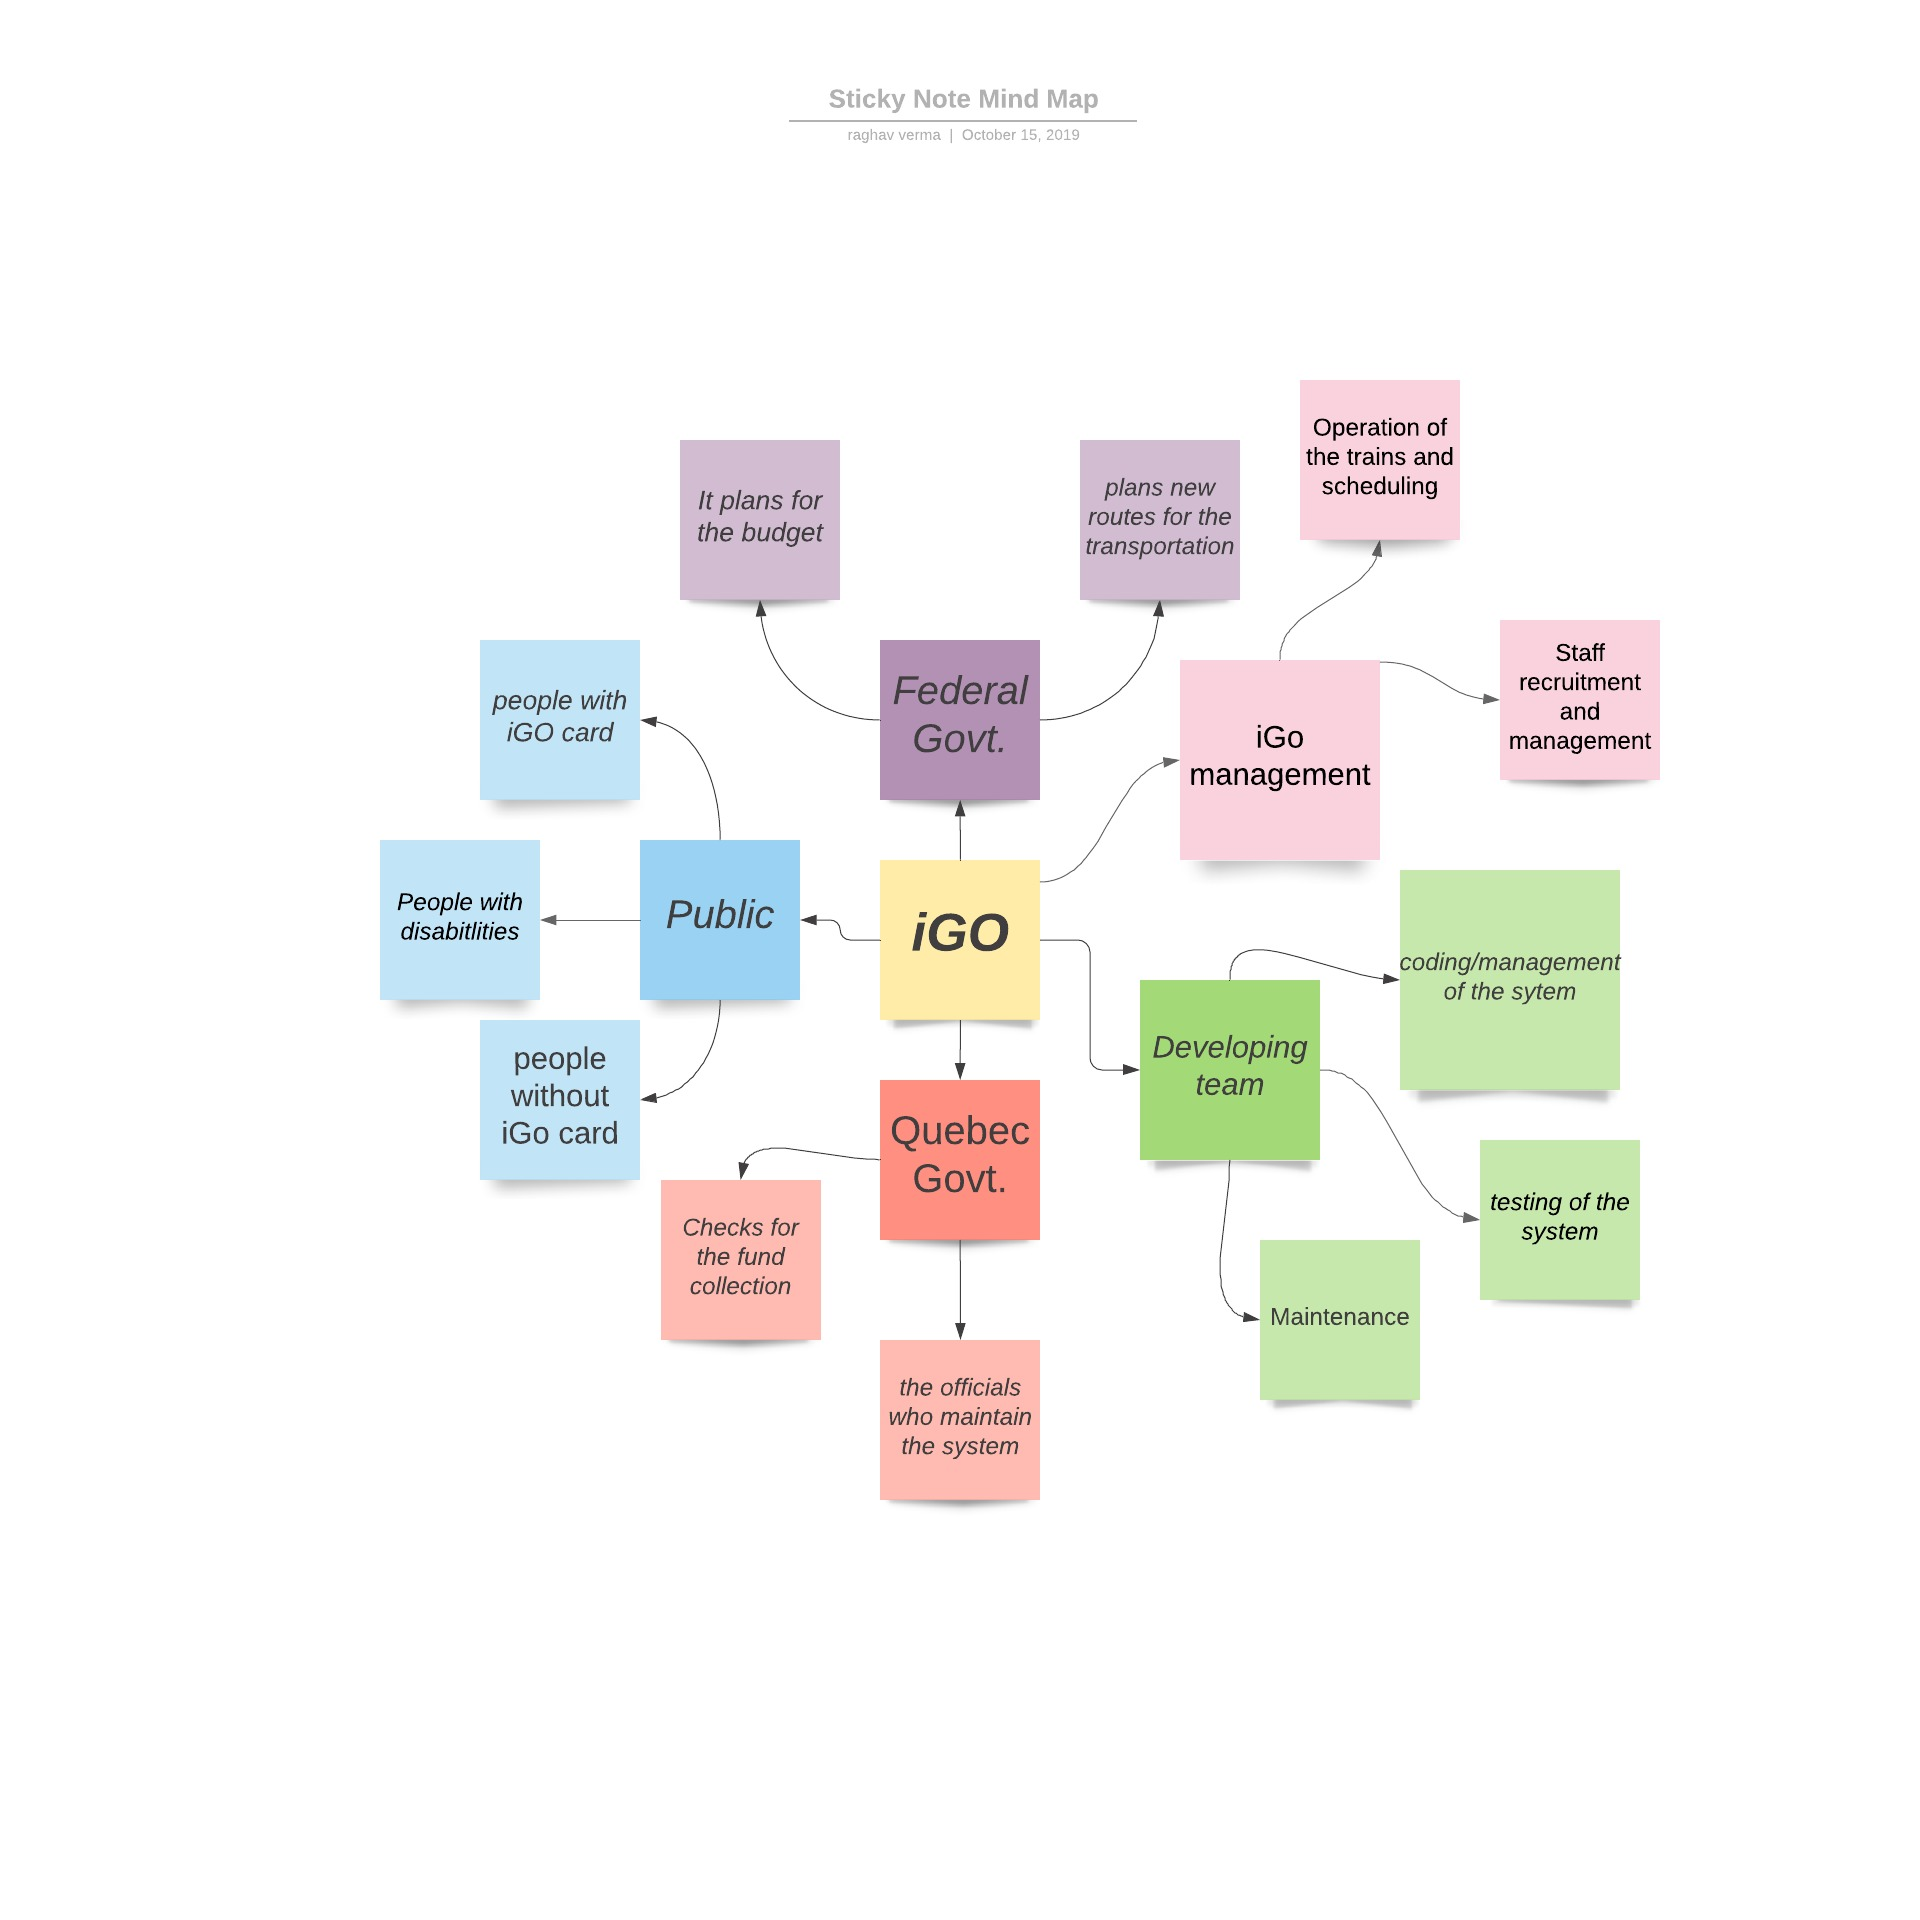
\includegraphics[width=450.75pt,height=486.75pt]{./p2_image2.jpeg}
	\end{Center}
  \caption{Mind map}
\end{figure}


%%%%%%%%%%%%%%%%%%%% Figure/Image No: 2 Ends here %%%%%%%%%%%%%%%%%%%%



\vspace{\baselineskip}
The following are the significant stakeholders for iGo project .[references: Domain modelling introduction:Kamthan]\par



\vspace{\baselineskip}
Direct users:\par

The direct users are the main consumer of the system iGo as they are the ones who will use the system for transportation and further users can be categorized among registered users(one with iG0 pass), no registered users and differently-able users.all the users which are registered,differently-able should be prioritise as important as they are the main consumer of the product and their satisfaction and feedback is highly important.\par


\vspace{\baselineskip}
Federal government and Quebec government:\par

The\ two governments should be prioritized as important as they maintain the budget for iG0 system and also plans and overview new routes for  iGo.the taxes are collected by both governments as collected from the iGo to maintain the budget.\par


\vspace{\baselineskip}

Business analysts:\par

They have the responsibility to check the iGo data, do the analysis of user data and thus analysing the collections made from the users.\par


\vspace{\baselineskip}
iGo management:\par

The representatives of iGo,managers, staff and operators are conclude as iGo management team and highly important and influential for the product\par


\vspace{\baselineskip}
iGo developrs:\par

The programmers and developers responsible for the development of the system taking into the considerations of design by the designers.\par


\vspace{\baselineskip}

iGo interface designers:\par

The designers who has the responsibility to meet the user satisfaction when they operate the iGo system and design the interface suitable for every type of direct users.\par

iGo testers:\par

The testers are responsible for regularly keeping the product in check and perform various tests to check for abnormalities.\par


\vspace{\baselineskip}
Equipment providers:\par
Rresponsible for providing the machines,paper,monitors, keypads,payments equipments,etc\par


\vspace{\baselineskip}
Financial institutions:\par

The banks have a significant role as the payments made are deposited into bank with iGo and also during the transactions,debit/credit cards are validated from the banks.\par


\vspace{\baselineskip}
\section{Negative stakeholders[2]}

These are the stakeholders which can degrade the overall quality and processing of iGo and also try to harm the any module of the system.\par


\vspace{\baselineskip}
Misusers:\par

there can be users who do not have their own cards but must be using cards of other users and thus enjoy the privileges of iGo.also the mis-users can make payments for transit fares by using fake/stolen credit cards.inspectors should be responsible for check the passes of doubtful passengers.\par


\vspace{\baselineskip}
Vandals:\par

the people who can destroy the iGo equipments or harm iGo management team. and such cases are not frequently occurring.anyway, security and inspectors should be regularly checking for such cases.\par


\printbibliography





\chapter{Problem Domain}
\begin{figure}[htb]

\begin{center}
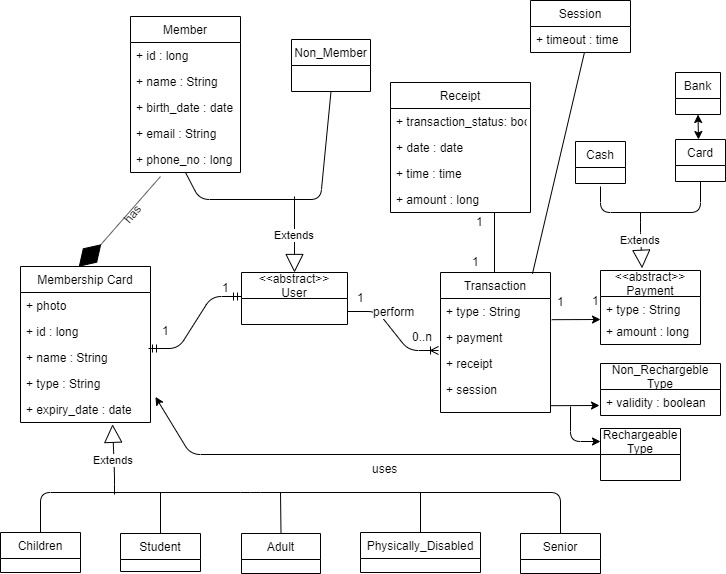
\includegraphics[scale=0.54]{./DomainModel}
\end{center}
\caption{UML Class Diagram}
\end{figure}
The problem domain of IGo system is represented by a set of concepts, properties and their relationships to each other. The concepts have been modelled as classes and their attributes represent the properties. The classes are also connected to each other and the connections have been labelled wherever relevant.

The central component of the IGo domain is the User class which has been made abstract as the user has to be a member or non-member of the STM service and cannot have an existence otherwise. Member user has attributes recorded as it will be used for the membership card\gls{membership_card} that he/she owns. The Membership Card class further is extended by 5 subclasses which depict the different types of cards allotted to users on the basis of age and other factors. Attributes of non-member user class are not relevant as he/she will be performing one-time transaction that does not make use of any registered passes.

The users interaction with IGo is represented as a Transaction  class which can be of two types : Non Rechargeable or Rechargeable purchase of ticket. If the user is performing a rechargeable transaction, they use the membership card they possess. In either case, payment will be made which is represented by the Payment class. The payment class is abstract as it should be either done through Card or Cash and do not have an independent existence otherwise. If using Card class, then authentication will be done thorough the Bank. Cash payments do not need authentication.

Every transaction provides a receipt indicating the date, time and status of transaction performed and the amount paid, which is represented by the Receipt class. Every transaction also creates a session\gls{session} as depicted by Session class which would expire after the time allotted, after which the transaction will be cancelled.

\chapter{Use Case Model}
\section{Use Case Diagram}
The UML Use Case Diagram can provide a high-level graphical representation of the actors, use cases, and their interactions. It also provides structural relationships between use cases, and structural relationships between actors.\\
\\
Based on the advantages of UML Use Case Diagram, this kind of diagram is chosen for modelling the iGo.\\
\\
The following diagram shows the basic use case diagram of iGo:
\begin{figure}[htb]
\centering
\begin{adjustwidth}{-2cm}{}
  \begin{tikzpicture}
    
	\begin{umlsystem}[x=3,y=0]{iGo System}
	\umlusecase[x=0,y=0,width=1cm,name=AT]{Access TVM}
	\umlusecase[x=3,y=2,width=3cm,name=AO]{Access OPUS card service}
	\umlusecase[x=3,y=-2,width=3cm,name=AN]{Access normal service}
	\umlusecase[x=6,y=0,width=2.5cm,name=ST]{Select ticket type}
	\umlusecase[x=10,y=2,width=2cm,name=VI]{View information}
	\umlusecase[x=10,y=0,width=2cm,name=CP]{Choose payment method}
	\umlusecase[x=7,y=-3,width=1cm,name=P1]{Pay by cc}
	\umlusecase[x=9,y=-3,width=1cm,name=P2]{Pay by db}
	\umlusecase[x=11,y=-3,width=1cm,name=P3]{Pay by cash}
	\umlusecase[x=9,y=-5,width=2cm,name=AP]{Authorize payment}
	\umlusecase[x=4.5,y=-4,width=2cm,name=APO]{Add pass on card}
	\umlusecase[x=4.5,y=-6,width=2cm,name=PT]{Print tacket}
	\umlusecase[x=0,y=-5,width=1.5cm,name=PR]{Print receipt}
	\end{umlsystem}
	
	\umlactor[x=0,y=0]{Traveller}
	\umlactor[x=16.5,y=-5]{Bank}
	
	\umlinclude{AT}{AN}
	\umlinclude{AO}{ST}
	\umlinclude{AN}{ST}
	\umlinclude{AO}{VI}
	\umlextend{AO}{AN}
	\umlextend{PR}{PT}
	\umlextend{PR}{APO}
	\umlassoc{ST}{CP}
	\umlassoc{P1}{AP}
	\umlassoc{P2}{AP}
	\umlassoc{P3}{AP}
	\umlassoc{AP}{APO}
	\umlassoc{AP}{PT}
	\umlinherit{P1}{CP}
	\umlinherit{P2}{CP}
	\umlinherit{P3}{CP}
	
	\umlassoc{Traveller}{AT}
	\umlassoc{Bank}{AP}

  \end{tikzpicture}
  \caption{Use case diagram of iGo System (UCMiGo)\gls{UCMiGo}}
\end{adjustwidth} 
\end{figure} 


\begin{figure}[htb]
  \centering
  \begin{tikzpicture}
  	\umlactor[x=6,y=0]{abstract Traveller}
  	\umlactor[x=3,y=-3]{citizen}
  	\umlactor[x=5,y=-3]{student}
  	\umlactor[x=7,y=-3]{senior}
  	\umlactor[x=9,y=-3]{disabled}
  	\umlinherit{citizen}{abstract Traveller}
  	\umlinherit{student}{abstract Traveller}
  	\umlinherit{senior}{abstract Traveller}
  	\umlinherit{disabled}{abstract Traveller}
  	
  \end{tikzpicture}
  \caption{Detail of abstract traveller actor}
\end{figure}

\section{Use case}
\begin{itemize}
	\item Access normal service\\
	The user access the normal TVM\gls{TVM} service without any using OPUS card, after successfully purchased, the TVM will give the user a ticket automatically.
	\item Access OPUS card service\\
	The user can also insert an OPUS card, instead of printing a ticket after purchased, the TVM will update the information of the OPUS card.
	\item View information\\
	The user can view information of their OPUS card after insertion, including the valid date of the card and in pass information.
	\item Authorize payment\\
	A secondary actor Bank is also take part in this use case, basically the Bank will check the validity of the card and charge fee based on the chosen ticket type if it pass the validity phase.
\end{itemize}

\section{Sequence Diagram of Making Payment}
\begin{figure}[htb]
\centering
  \begin{tikzpicture}
  \begin{umlseqdiag}
    \umlactor[scale=0.5,no ddots]{Traveller}
    \umlobject[no ddots]{iGo}
    \umlobject[no ddots]{STM}
    \umlobject[no ddots]{Bank}
    \begin{umlcall}[op=check TVM validity,type=asynchron]{Traveller}{iGo}
      \begin{umlcall}[op=give respond,type=asynchron]{iGo}{Traveller}
      \end{umlcall}
    \end{umlcall}
    \begin{umlfragment}
    \begin{umlcall}[op=insert card,type=synchron,return=show card info]{Traveller}{iGo}
      \begin{umlcallself}[op=process,type=asynchron]{iGo}
      \end{umlcallself}
    \end{umlcall}
    \end{umlfragment}

  \end{umlseqdiag}
  \end{tikzpicture}
  \caption{First part of the sequence diagram}
 \end{figure}
 
 \begin{figure}[htb]
   \centering
   \begin{tikzpicture}
     \begin{umlseqdiag}
     \umlactor[scale=0.5,no ddots]{Traveller}
     \umlobject[no ddots]{iGo}
     \umlobject[no ddots]{STM}
     \umlobject[no ddots]{Bank}
      \begin{umlcall}[op=select ticket type,type=asynchron]{Traveller}{iGo}
      \begin{umlcall}[op=select payment method,type=synchron]{Traveller}{iGo}
        \begin{umlcall}[op=send request,type=synchron,return=respond with link]{iGo}{STM}
          \begin{umlcallself}[op=verify,type=asynchron]{STM}
          \end{umlcallself}
        \end{umlcall}
        \begin{umlcall}[op=respond with link,type=return]{iGo}{Traveller}
        \end{umlcall}
        \begin{umlcall}[op=provide payment details,type=synchron,return=return purchase info]{Traveller}{iGo}
          \begin{umlcall}[op=process payment,type=synchron]{iGo}{Bank}
            \begin{umlcall}[op=valid card info,type=asynchron]{Bank}{Bank}
            \end{umlcall}
            \begin{umlfragment}[type=alt,label=info valid]
              \begin{umlcallself}[op=charge fee,type=asynchron]{Bank}
              \end{umlcallself}
              \begin{umlcall}[op=authorized,type=return]{Bank}{STM}
                \begin{umlcallself}[op=update info,type=asynchron]{STM}
                \end{umlcallself}
                \begin{umlcall}[op=update success,type=return]{STM}{iGo}
                \end{umlcall}
              \end{umlcall}
              \umlfpart[else]
              \begin{umlcall}[op=reject,type=return]{Bank}{STM}
                \begin{umlcall}[op=update fail,type=return]{STM}{iGo}
                \end{umlcall}
              \end{umlcall}
            \end{umlfragment}
          \end{umlcall}
        \end{umlcall}
      \end{umlcall}
    \end{umlcall}
     \end{umlseqdiag}
   \end{tikzpicture}
   \caption{Second part of the sequence diagram}
 \end{figure}
\section{Positive Scenarios}
\begin{figure}[htb]
  \centering
  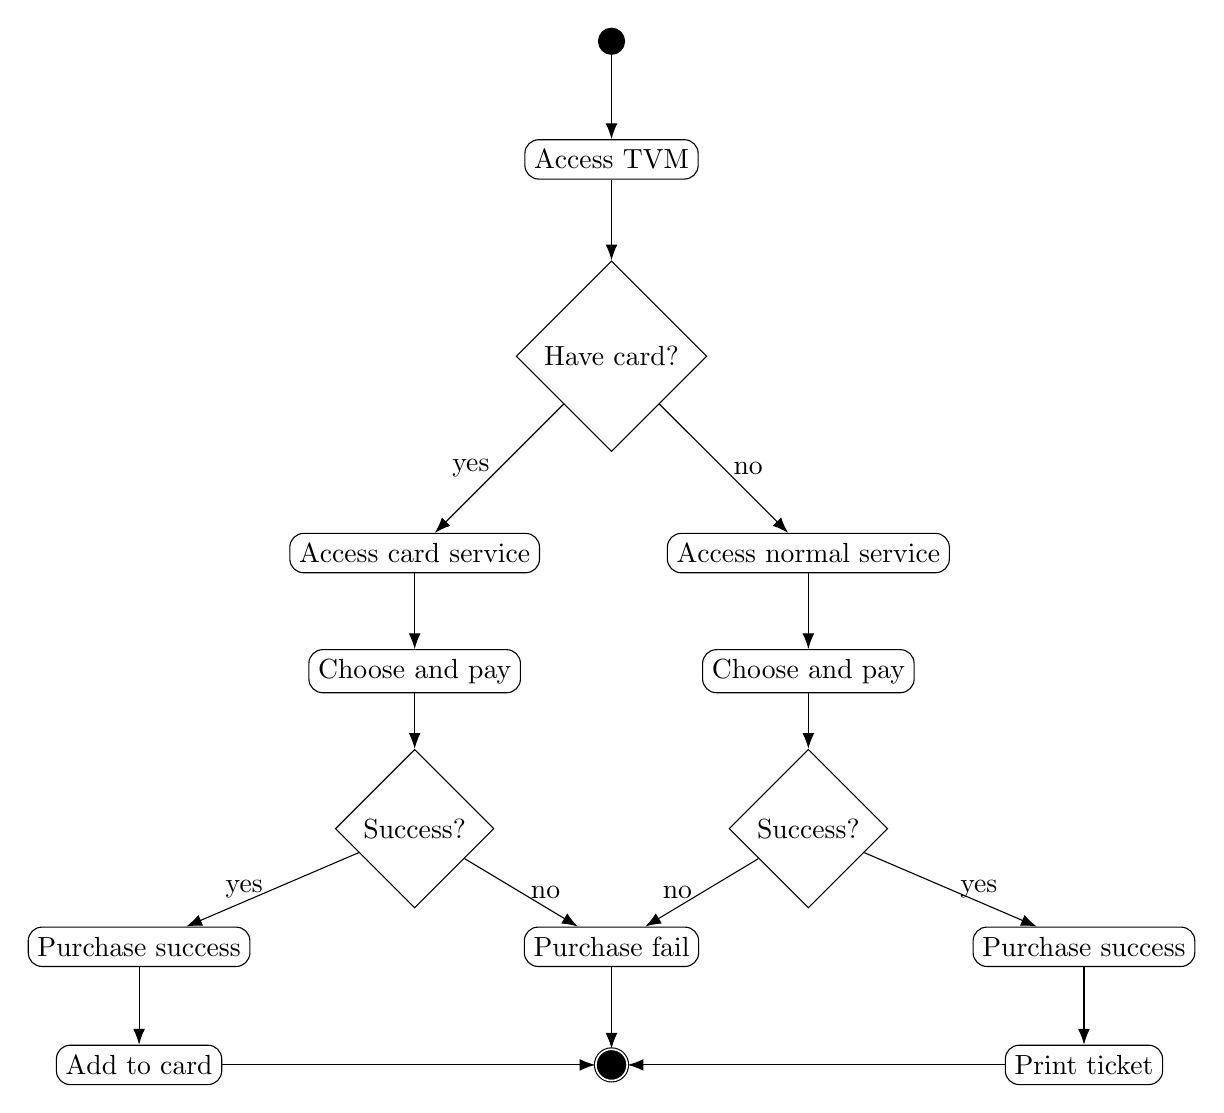
\begin{tikzpicture}
    \tikzset{start/.style={circle,minimum width=0.3cm ,minimum height=0.3cm, draw ,fill}}
    \tikzset{activity/.style={rectangle,minimum width=1cm ,minimum height=0.5cm,rounded corners =5pt,draw}}
    \tikzset{end/.style ={draw ,double =white , circle ,inner sep =4pt , minimum width =0.3 cm , minimum height =0.3cm,draw,fill}}
    \tikzset{decision/.style ={diamond,minimum width=0.2cm ,minimum height=0.2cm , draw}}
    \draw (0,0) node[start](start){};
    \draw (0,-1.5) node[activity](a1){Access TVM};
    \draw (0,-4) node[decision](d1){Have card?};
    \draw (-2.5,-6.5) node[activity](a2){Access card service};
    \draw (2.5,-6.5) node[activity](a3){Access normal service};
    \draw (-2.5,-8) node[activity](a4){Choose and pay};
    \draw (2.5,-8) node[activity](a5){Choose and pay};
    \draw (-2.5,-10) node[decision](d2){Success?};
    \draw (2.5,-10) node[decision](d3){Success?};
    \draw (0,-11.5) node[activity](a6){Purchase fail};
    \draw (0,-13) node[end](e1){};
    \draw (-6,-11.5) node[activity](a7){Purchase success};
    \draw (6,-11.5) node[activity](a8){Purchase success};
    \draw (-6,-13) node[activity](a9){Add to card};
    \draw (6,-13) node[activity](a10){Print ticket};
    \draw[->](start) -- (a1);
    \draw[->](a1) -- (d1);
    \draw[->](d1) -- node[left]{yes}(a2);
    \draw[->](d1) -- node[right]{no}(a3);
    \draw[->](a2) -- (a4);
    \draw[->](a3) -- (a5);
    \draw[->](a4) -- (d2);
    \draw[->](a5) -- (d3);
    \draw[->](d2) -- node[left]{yes}(a7);
    \draw[->](d2) -- node[right]{no}(a6);
    \draw[->](d3) -- node[left]{no}(a6);
    \draw[->](d3) -- node[right]{yes}(a8);
    \draw[->](a6) -- (e1);
    \draw[->](a7) -- (a9);
    \draw[->](a8) -- (a10);
    \draw[->](a9) -- (e1);
    \draw[->](a10) -- (e1);
    
  \end{tikzpicture}
  \caption{Scenarios}
\end{figure}

\chapter{Conclusion}
The document describes in detail the working and features of the iGO ticket vending machine with respect to the stakeholder's usage of it, which is also graphically depicted in the Mind map of the stakeholders, UML class diagram, Use Case diagram and the sequence diagram of the system.
\clearpage



\printglossaries
\clearpage
\LARGE \textbf {Reference}\normalsize
\begin{enumerate}
\item Alonso-Ríos, Vázquez-García, Mosqueira-Rey, Moret-Bonillo,2010; Alonso-Ríos, Mosqueira-Rey, Moret-Bonillo, 2018\\
https://www.tandfonline.com/doi/full/10.1080/10447318.2018.1424101
\item use\_case\_modeling\_negative,Kamthan \\
\item Use Case Modeling, Dr. Pankaj Kamthan, Concordia University \\ 
\item Brainstorming and MindMapping, Dr. Pankaj Kamthan, Concordia University \\
\item STM  http://www.stm.info/en \\
\end{enumerate}
\end{document}